\chapter{Conceitos teóricos}
\label{cha:conceitos_teoricos}

\section{Sensor - GPS}
\label{sec:gps}

O Sistema de Posicionamento Global (GPS – Global Positioning System) é uma rede utilizada mundialmente pela população para determinação da localização na superfície do globo terrestre. 
Este sistema tem o nome de Navstar e é financiado e gerido pelo Departamento da Defesa dos Estados Unidos da América.
Este é um dos vários sistemas de posicionamento existentes mundialmente, pois existem também os sistemas GLONASS da Rússia, o COMPASS desenvolvido pela China e o GALILEO da União Europeia, cada um deles com diferentes níveis de desenvolvimento e testes.
Apesar de ter sido desenvolvido para fins militares, em 1983 foi permitida a sua utilização por parte de civis, sendo que na época o sinal era degradado e continha um erro de +/- 100 metros, algo que foi eliminado no ano de 2010.
Os satélites GPS transmitem sinais para os recetores GPS, os quais são elementos passivos no sistema pois não transmitem qualquer tipo de informação, tornando-se este um sistema de comunicação unilateral.
Este serviço de localização necessita de uma visão desimpedida do céu e apenas no exterior consegue apresentar bons resultados, os quais dependem de relógios atómicos presentes nos satélites que proporcionam ao sistema a sua elevada precisão.
Cada satélite GPS transmite informação relativa ao seu posicionamento relativo ao planeta, bem como a hora atual.
Todas as operações realizadas pelos satélites encontram-se sincronizadas para que o seu sinal constante seja transmitido nos mesmos instantes de tempo.
Os sinais emitidos pelos satélites são enviados à velocidade da luz para os recetores GPS e utilizando o tempo de percurso desse sinal é possível determinar a distância a que cada satélite se encontra do recetor.
Assim que o recetor ler a informação de pelo menos quatro satélites é possível calcular a sua posição em três dimensões.
A todo o momento existem pelo menos 24 satélites GPS em funcionamento que realizam duas órbitas por dia a uma altura de 18 500 km e a uma velocidade próxima de 14 000 km/h.
Cada recetor recebe informação sobre o local em que um satélite se encontra num determinado momento do dia e com essa informação consegue determinar que se encontra algures numa superfície esférica em que o centro é o próprio satélite.
Cruzando os pontos de pelo menos quatro satélites, o recetor determina o local em que todas as esferas se intersectam e desta forma concluí a sua própria posição com um erro de +/- 10 m.

\begin{figure}[hbtp]
	\centering
	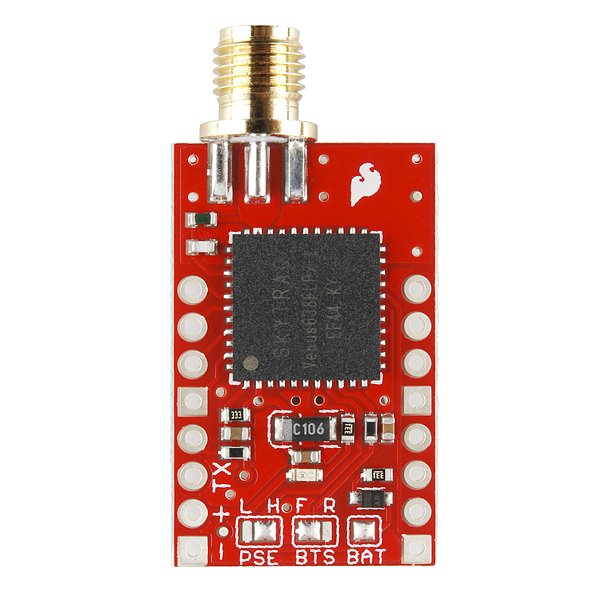
\includegraphics[width=7cm]{venus}
	\caption[Sensor Venus638FLPx]{Sensor Venus638FLPx \footnotemark}
	\label{fig:sensor_venus638FLPx}
\end{figure}

\footnotetext{http://www.sparkfun.com/products/11058}

O recetor GPS utilizado foi o Venus638FLPx que recebe mensagens normalizadas NMEA (explicada em ~\ref{sub:nmea}) a uma taxa padrão de 9600 bps que pode ser alterada para 115200 bps e é alimentado a uma tensão de 3.3 V.
Por definição padrão, este recetor GPS recebe cinco tipos de mensagens NMEA, das quais apenas uma é utilizada neste projeto, pois apenas ela refere todos os valores desejados obter: latitude, longitude, data e hora.
Uma mensagem do tipo RMC tem o aspeto da figura \ref{fig:formato_de_mensagem_rmc} sendo que a tabela \ref{tab:nmea_rmc} descreve o seu significado.

\begin{figure}[hbtp]
	\centering
	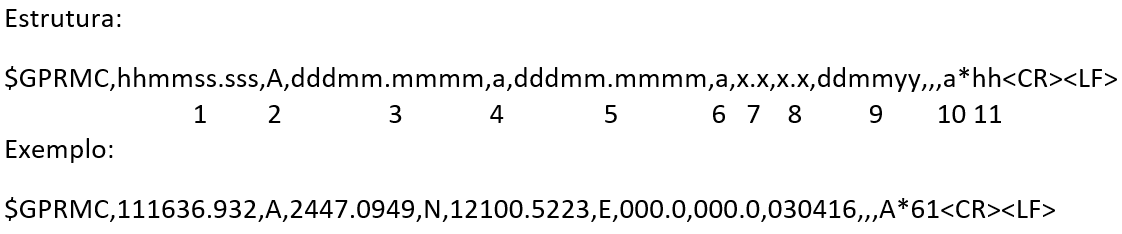
\includegraphics[width=14.5cm]{GPRMC}
	\caption{Formato de mensagem RMC}
	\label{fig:formato_de_mensagem_rmc}
\end{figure}

Foi também necessário fazer algumas configurações, utilizando um conjunto de mensagens que o recetor conseguisse entender.
Todas as mensagens têm o formato apresentado na figura \ref{fig:formato_de_mensagem_de_configuracao_do_recetor_gps}, em que o campo <CC> representa o código da mensagem e <BB> a informação a transmitir nessa mensagem.
As mensagens enviadas tinham os códigos ``05'' e ``09'', referentes à velocidade de comunicação do GPS e ao tipo de mensagem que o GPS deve ler, respetivamente.
Toda esta informação foi retirada diretamente do datasheet do recetor Venus638FLPx.

\begin{figure}[hbtp]
	\centering
	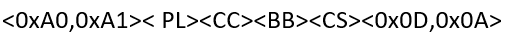
\includegraphics[width=7cm]{mensagemgps}
	\caption{Formato de mensagem de configuração do recetor GPS}
	\label{fig:formato_de_mensagem_de_configuracao_do_recetor_gps}
\end{figure}

\begin{table}[hbtp]
\centering
\caption{Interpretação dos dados de uma mensagem NMEA do tipo RMC}
\label{tab:nmea_rmc}
\begin{tabular}{|c|l|l|l|}
\hline
\multicolumn{1}{|l|}{Campo} & Nome & Exemplo & Descrição \\ \hline
1 & Tempo UTC & 111636.932 & \begin{tabular}[c]{@{}l@{}}Tempo UTC no formato hhmmss.sss\\ (000000.000 $\sim$235959.999)\end{tabular} \\ \hline
2 & Estado & A & \begin{tabular}[c]{@{}l@{}}Estado: 'V' - Aviso na receção de dados\\              'A' - Dados válidos\end{tabular} \\ \hline
3 & Latitude & 2447.0949 & Latitude no formato ddmm.mmm \\ \hline
4 & Indicador N/S & N & \begin{tabular}[c]{@{}l@{}}Indicador de hemisfério: 'N' - Norte\\                                          'S' - Sul\end{tabular} \\ \hline
5 & Longitude & 12100.5223 & Longitude no formato dddmm.mmm \\ \hline
6 & Indicador E/W & E & \begin{tabular}[c]{@{}l@{}}Indicador de hemisfério: 'E' - Este\\                                         'W' - Oeste\end{tabular} \\ \hline
7 & Velocidade no solo & 000.0 & Velocidade no solo em nós \\ \hline
8 & Percurso no solo & 000.0 & Direção de deslocação em graus \\ \hline
9 & Data UTC & 030416 & Data UTC no formato ddmmyy \\ \hline
10 & Indicador de modo & A & \begin{tabular}[c]{@{}l@{}}Indicador de modo:\\ 'N' - Data inválida\\ 'A' - Modo autónomo\\ 'D' - Modo diferencial\\ 'E' - Modo de estimativa\\ 'M' - Modo manual\\ 'S' - Modo de simulação\end{tabular} \\ \hline
11 & Confirmação & 61 & \begin{tabular}[c]{@{}l@{}}Número de caracteres enviados\\ pelo satélite\end{tabular} \\ \hline
\end{tabular}
\end{table}
\FloatBarrier

\subsection{NMEA}
\label{sub:nmea}

NMEA é a sigla de National Marine Electronics Association (Associação Nacional de Eletrónica dos Marines) desenvolveu uma especificação que define a interface entre vários elementos do equipamento desta forma militar norte-americana.
A receção de comunicação GPS está englobada nesta especificação e a maioria dos programas desenhados para fornecer dados sobre posicionamento em tempo real estão desenhados para obter informação neste formato.
A informação fornecida por este serviço incluí posição, velocidade e tempo e esta informação é enviada em formato de uma frase, iniciada sempre com o caracter '\$', é procedida pelo prefixo GP (relativo a posicionamento global) e ainda por três letras que identificam o tipo de mensagem que é recebida.
Cada frase é terminada com um caracter de fim de linha e retorno e a informação contida em cada mensagem está separada por vírgulas, tal como indicado na figura \ref{fig:formato_de_mensagem_rmc}.

\section{Sensor - Acelerómetro}
\label{sec:acelerometro}

Um acelerómetro é um dispositivo que mede a aceleração a que está sujeito, no caso de se encontrar estacionário na superfície terrestre, este dispositivo sofre uma aceleração vertical de 9,8 m/s$^2$ e caso se encontre em queda livre mede uma aceleração de 0 m/s$^2$.
Por este valor ser o valor constante de aceleração gravítica, foi criada uma unidade de medida ``g'' para mais facilmente expressar valores de aceleração, sendo que 1 g equivale a 9,8 m/s$^2$.
Os acelerómetros têm diversas aplicações na indústria e na ciência devido à sua elevada sensibilidade e são regularmente utilizados para detetar vibrações em diversas máquinas, em telemóveis e tablets e também em aeronaves, incluindo drones, para uma melhor estabilização de voo.
Conceptualmente, um acelerómetro comporta-se como uma massa amortecida por uma mola, sendo possível determinar o valor de aceleração sabendo o peso da massa e a constante de elasticidade da mola.
Em termos práticos um acelerómetro pode utilizar vários métodos para determinar as suas leituras mas os dois mais comuns são os acelerómetros piezoelétricos e os capacitivos.
Acelerómetros piezoelétricos medem aceleração diretamente proporcional a uma força a partir de certos tipos de cristais.

\begin{figure}[hbtp]
	\centering
	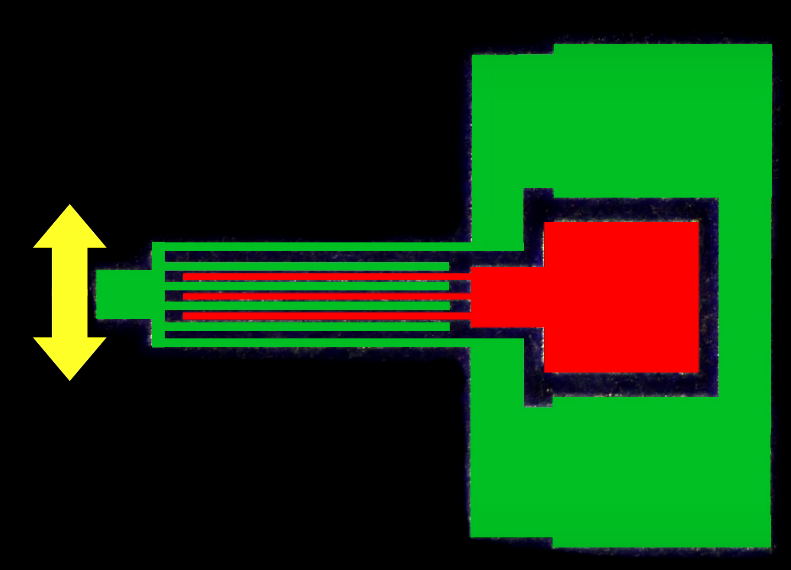
\includegraphics[height=5cm]{capacitivo}
	\caption[Ilustração de um acelerómetro capacitivo]{Ilustração de um acelerómetro capacitivo \footnotemark}
	\label{fig:capacitivo}
\end{figure}
\footnotetext{https://www.youtube.com/watch?v=i2U49usFo10}

Estes cristais, quando comprimidos, deslocam as cargas existentes no seu interior e consequentemente alteram o seu valor resistivo que pode ser traduzido para uma variação de corrente ou tensão e que pode ser medida.
Já os acelerómetros capacitivos (\ref{fig:capacitivo}) utilizam um sistema semelhante ao de um condensador.
São compostos por duas zonas eletricamente condutoras e isoladas uma da outra que contêm alguma carga.
A separação entre estas zonas é tão pequena, que quando existe algum movimento, a distância entre ambas é alterada, alterando assim o valor de capacitância do sistema, que se traduz facilmente para uma variação de tensão.
Para este projeto foi utilizado um acelerómetro ADXL345 capacitivo, capaz de medir variações de aceleração até  $\pm$ 16g.
Para a sua utilização foi necessário determinar a velocidade de transmissão com o valor de 9600 bps, tal como os restantes dispositivos do sistema e também a frequência de amostragem de valores, nomeadamente 200 Hz.
Para a comunicação foi utilizado o método I$^2$C todavia, estava também disponível a opção de transmissão por SPI, sendo que a escolha foi tomada devido a serem necessárias menos ligações em I$^2$C.
Apesar da comunicação SPI suportar velocidades de transmissão mais elevadas, esta vantagem não se mostra relevante a 200 Hz.
O acelerómetro em questão oferece uma biblioteca de funções de teste, entre as quais a deteção de queda livre, toque simples e toque duplo que, apesar de não serem utilizadas no projeto, foram bastante importantes aquando da aprendizagem de utilização do dispositivo.
Para que fosse possível obter os valores de leitura do acelerómetro, foi necessário ler os valores entre os registos 50 e 55, sendo que cada par contém informação sobre um dos três eixos de deslocação.
Os valores lidos foram então estudados utilizando um gráfico, sendo que a sua análise está descrita na secção \ref{fig:grafico_de_uma_irregularidade_detetada}.

\section{Comunicação - Bluetooth}
\label{sec:bluetooth}

Bluetooth é um padrão de tecnologia sem fio utilizada para troca de dados a curtas distâncias que utiliza ondas rádio UHF, nomeadamente com a utilização de uma frequência que se encontra entre 2400 e 2480 MHz.
Esta tecnologia permite a ligação entre vários dispositivos, até um máximo de sete, sendo uma das primeiras tecnologias a surgir que permitiu a ligação entre mais de dois dispositivos.
A tecnologia Bluetooth é gerida pelo Grupo de Interesse Especial (SIG - Special Interesse Group em inglês) e conta com a colaboração de mais de 30.000 empresas parceiras, que têm atividade nas áreas de telecomunicação, computação e redes.
O sistema Bluetooth divide os dados que deseja enviar em pacotes e transmite cada um desses pacotes num dos 80 canais Bluetooth, cada um deles com uma largura de banda de 1 MHz, alternando a seleção de cada canal cerca de 800 vezes por segundo, utilizando a tecnologia AFH - Adaptive Frequency Hopping.
Existe também um modo de baixo consumo que utiliza canais de 2 MHz, o que faz um total de 40 canais.
Este sistema funciona assente numa estrutura master-slave, em que um mestre (ou dispositivo primário) pode comunicar com um máximo de sete escravos (ou dispositivos secundários), sendo que todos os escravos estão sincronizados com o mestre, através do seu relógio interno.
O relógio do mestre conta intervalos de tempo de $312,5 \mu s$, juntando dois intervalos de tempo para fazer intervalo de comunicação de $625 \mu s$.
A sequência destes intervalos de comunicação determina que o mestre transmite nos intervalos pares e recebe informação nos ímpares e por analogia o escravo recebe nos intervalos pares e envia nos ímpares.
É também de salientar que um dispositivo dentro de um sistema não é sempre escravo ou mestre, pois pode mudar o seu estatuto, dependendo da funcionalidade que lhe é atribuída e que um escravo pode ter mais que um mestre.

\begin{figure}[hbtp]
	\centering
	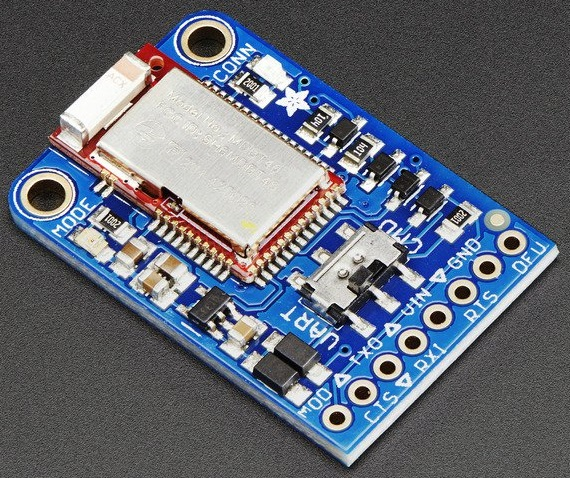
\includegraphics[height=5cm]{bluetooth}
	\caption[Módulo bluetooth]{Módulo bluetooth \footnotemark}
	\label{fig:modulo_bluetooth}
\end{figure}
\footnotetext{https://www.adafruit.com/product/2479}

O padrão de Bluetooth tem uma ligação direta entre potência e alcance e esse alcance determina em que classe de dispositivo rádio o transmissor se encontra.
Um transmissor de classe 3 tem um alcance até 1 metro e consome o máximo de 1 mW.
Para transmissores de classe 2, o alcance vai até 10 metros, levando a um consumo máximo de 2,5 mW.
Por último, a classe 1 tem transmissores com alcance máximo de 100 metros, sendo consumidos até 100 mW.
O sistema Bluetooth encontra-se principalmente na classe 2 mas versões mais atuais conseguem por vezes alcançar a classe 1, com um alcance de 60 metros.
No que diz respeito ao dispositivo utilizado, foi um HC-06 \ref{fig:modulo_bluetooth} série que não necessitou de qualquer tipo de configuração uma vez que a frequência de transmissão pré-definida é de 9600 bps.
Foi apenas necessário alimentar este dispositivo e quando era estabelecida a ligação, uma palavra-passe tinha que ser introduzida, neste caso, ``1234''.

\section{Comunicação - Wi-Fi}
\label{sec:wi-fi}

Wi-Fi é uma tecnologia de ligação local sem fios baseada nos padrões IEEE 802.11, uma norma que regula a comunicação sem fios em determinadas frequências rádio.
Entre os dispositivos que utilizam esta tecnologia estão os computadores, consolas de jogos, tablets e telemóveis e também impressoras, mas outros dispositivos como televisões e automóveis começam também a integrar esta tecnologia.
A ligação à Internet pode ser feita através de WLAN, uma rede local que usa ondas de rádio, através de um \emph{router}, dispositivo que obtém ligação à Internet via cabo Ethernet.
Como esta tecnologia opera em frequências que não necessitam de licença, o apelo à sua utilização é bastante elevado, sendo apenas necessário equipamento homologado pela entidade responsável do país vendedor do dispositivo, que usualmente segue normas internacionais.
A tecnologia Wi-Fi utiliza habitualmente as frequências de 2,4 GHz e 5 GHz e tem um alcance médio de 20 metros para interiores, caso não existam obstáculos pelo caminho, como paredes, o que pode limitar o alcance a apenas uma sala.
No que toca ao exterior, a cobertura Wi-Fi pode atingir vários quilómetros caso sejam utilizados repetidores de sinal, normalmente instalados com grandes antenas.
A certificação dos dispositivos Wi-Fi é feita pela aliança Wi-Fi, um conjunto de entidades espalhadas por todo o mundo que garantem a utilização do protocolo 802.11 definido pelo IEEE, bem como os padrões de segurança WPA e WPA2 e o padrão de autenticação EAP.

Existem também pontos de acesso espalhados por várias cidades, que fornecem uma rede gratuita para os cidadãos, nomeadamente em Lisboa e em Sintra, assim como em universidades, através da rede Eduroam, comum à maioria das universidades portuguesas, permitindo o acesso a qualquer estudante, independentemente da universidade em que esteja, mesmo não sendo estudante nesse estabelecimento de ensino.
Quanto ao nível de interferências, existem bastantes, graças à existência de vários pontos de acesso que sobrepões as suas redes, assim como pela utilização das mesmas frequências por outras comunicações como o Bluetooth ou o ZigBee.
Ainda assim, estas interferências são usualmente colmatadas com a rápida transmissão de dados, sendo que informação não recebida é rapidamente reenviada.
Outro mecanismo de redução de interferências é o SSID, um identificador de serviço que permite identificar o emissor e recetor de determinada informação.

\section{Comunicação - Redes móveis (3G)}
\label{sec:3g}

3G, abreviatura de terceira geração, é a terceira geração de tecnologia de telecomunicações móveis sem fios e assenta num conjunto de normas e serviços de utilização de telecomunicações móveis, cumprindo normas IMT-2000.
Esta tecnologia tem como principais focos a realização de chamadas por telemóveis, o acesso à Internet sem fios e também transmissão de televisão sem fios.
Estas redes permitem a transferência de informação a velocidades sempre superiores a 200 Kbps e podem atingir velocidades de vários Mbps, uma velocidade bastante elevada na área de comunicação sem fios.
Gerações anteriores a esta foram criadas no inicio dos anos 80 e cada nova geração surge com espaçamentos de cerca de 10 anos.
Esta tecnologia, apesar de ter processos bastante diferentes da Wi-Fi, apresenta resultados semelhantes, pois permite a ligação à Internet através de um telemóvel, tornando possível o envio dos dados recolhidos pelo acelerómetro para uma página \emph{web}.

\section{Processamento - Arduino}
\label{sec:arduino}

O Arduino é uma plataforma \emph{open-source} utilizada  para projetos de eletrónica que contém um micro-controlador programável através de um \emph{software} dedicado.
Esta plataforma é muito popular devido à sua facilidade de programação, tanto pela linguagem utilizada (C++) como pelo \emph{hardware} em si, uma vez que é apenas necessário ligar a placa ao computador via USB.
Um dos seus pontos fortes está na capacidade de poder interagir com botões, motores, câmeras, \emph{LEDs}, telemóveis, entre tantas outras coisas.
Esta diversidade, aliada  ao baixo custo do sistema, tem levado aos crescimento da comunidade que, contribui com código e instruções de utilização para diversos projetos desenvolvidos.
A placa mais comum é o Arduino Uno mostrado na figura \ref{fig:arduino}, pois contém um número de pins suficiente para construir a maior parte dos projetos iniciais, sendo que para projetos mais avançados são normalmente utilizados o Arduino Nano, devido ao seu pequeno tamanho, e o Arduino Mega que tem mais pins e um maior poder de processamento.
Todas as placas têm pins em comum entre si, alterando a quantidade desses pins dependendo do tamanho da placa.
O Arduino pode ser alimentado via USB ou através de um conector que forneça uma tensão dentro de limites específicos, normalmente entre 7 e 12 V.
Existem também os pins GND para ligação à massa, 5V e 3.3V, que fornecem alimentação com esses valores, Analog e Digital, utilizados para ligação de sensores analógicos e digitais, respetivamente.
Existe também um botão de reset que faz o código reiniciar, para que seja possível fazer múltiplos testes sem que seja necessário desconectar a alimentação.
Por fim, existe um conjunto de LEDs de controlo para ajudar o utilizador a saber o estado do seu projeto.
O LED ``power'' indica se existe uma alimentação correta ao Arduino e os LEDs ``Rx'' e ``Tx'' fornecem informação relativa à comunicação série do Arduino com outros equipamentos, nomeadamente ``Rx'' acende quando a placa recebe informação e ``Tx'' acende quando é enviada informação.

\begin{figure}[hbtp]
	\centering
	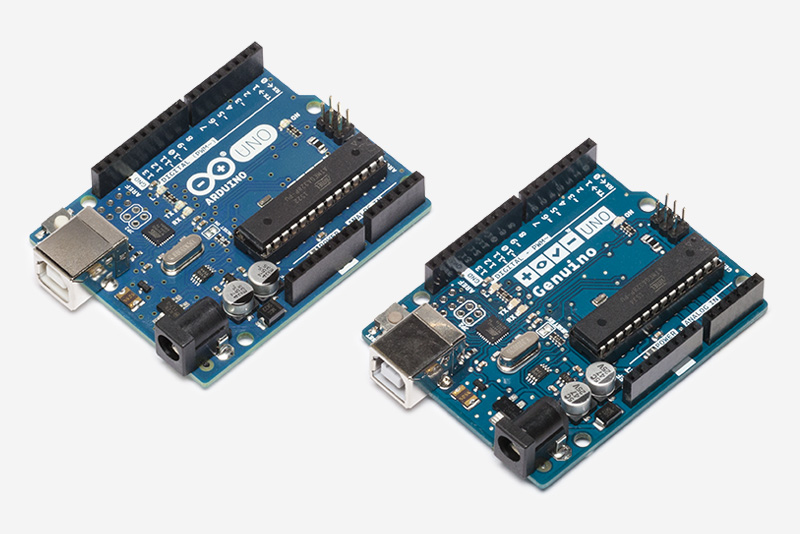
\includegraphics[height=5cm]{Arduino}
	\caption[Arduino Uno]{Arduino Uno \footnotemark}
	\label{fig:arduino}
\end{figure}
\footnotetext{http://www.arduino.cc/en/Main/ArduinoBoardUno}

\section{Processamento - Android}
\label{sec:android}

O sistema Android é um sistema operativo para telemóveis desenvolvido pela Google, que utiliza Linux na sua base e tem como principal objetivo o desenvolvimento de aplicações para telemóveis e tablets que disponham de ecrã táctil.
Nestes ecrãs é possível detetar diversos gestos como deslizar, bater e apertar, de modo a manipular objetos que estejam visíveis no ecrã, dando também a possibilidade de utilizar o teclado existente no ecrã.
É também possível adicionar outros componentes de hardware para controlar as aplicações, através de ligação USB ou Bluetooth, de modo a aumentar as possibilidades de interação com o utilizador.
O sistema Android dispõe também de um sistema televisivo, automóvel e de relógios, que ainda se encontram numa fase de desenvolvimento inicial mas apresentam resultados promissores.
De modo a fazer uma melhor leitura dos gestos que o utilizador realiza, o sistema Android é também capaz de ler informação de acelerómetros, giroscópios ou recetores GPS que façam parte do telemóvel, dando respostas visuais pelo ecrã mas também sensoriais ao nível do som e vibração do dispositivo.
O ecrã inicial do Android utiliza atalhos e \emph{widgets}, sendo que um atalho inicia a aplicação referente enquanto que um \emph{widget} fornece informação em tempo real, como o estado do tempo ou emails que sejam recebidos pelo utilizador.
No cimo deste ecrã inicial existe uma barra que fornece informação sobre o dispositivo e as suas conexões, que pode ser arrastada para baixo, expondo informação relevante sobre as aplicações, atualizações e até algumas definições que sejam habitualmente alteradas como o brilho do ecrã ou a ligação à Internet.

\subsection{Aplicações}
\label{sub:aplicacoes}

As aplicações são o que possibilitam uma utilização mais complexa de um dispositivo com o sistema operativo Android instalado.
Estas são normalmente desenvolvidas em Java mas podem ser combinadas com código C ou C++.
A programação destas aplicações é feita num SDK (software de desenvolvimento) que normalmente inclui ferramentas de desenvolvimento, um detetor de erros, algumas bibliotecas, um compilador e um emulador, para que seja possível simular a utilização de um telemóvel no computador.
Entre os mais comuns estão o Eclipse, o Android Studio e o MIT App Inventor.
O ambiente de programação Eclipse necessita da instalação de um extra para que seja possível o desenvolvimento de código para Android e era o ambiente de desenvolvimento oficial até 2014.
No final de 2014, a Google apresentou o Android Studio: um programa dedicado ao desenvolvimento Android que contém todas as opções existentes no universo Android, sendo este o principal ambiente de desenvolvimento.
Existe também o MIT App Inventor, que corre num \emph{browser web} e permite o desenvolvimento de aplicações sem que seja escrito código, utilizando a programação por módulos que se ligam entre si, não exigindo uma capacidade de processamento tão alta como o Android Studio.
Para que uma aplicação possa ser executada no telemóvel, é necessário instalar o ficheiro APK da aplicação, através da loja ``Google Play'' ou diretamente por ligação USB a um computador, permitindo a qualquer utilizador o desenvolvimento da sua própria aplicação, o seu teste e partilha.
O sistema operativo Android é baseado em Linux, com bibliotecas, API's e algum software escrito em C e ainda algumas traduções de bibliotecas para Java que torna possível a execução das aplicações.
Estas bibliotecas em Java são originárias e programadas a partir do OpenJDK, uma ferramenta que contém uma máquina virtual, as suas próprias bibliotecas e também um compilador.
Em termos específicos desta dissertação, a escolha do sistema operativo Android foi simples, uma vez que existem cerca de 86\% de utilizadores do sistema Android no universo dos telemóveis.
Além disso, as ferramentas para desenvolvimento de aplicações Android são mais acessíveis do que para iOS, o segundo sistema operativo mais frequente em telemóveis.

\section{Linguagem de programação - C}
\label{sec:C}

A linguagem de programação C foi uma das primeiras a surgir e uma das mais utilizadas no ramo das linguagens de baixo nível.
Em C, todo o código executável está contido em sub-rotinas denominadas funções, que podem ter parâmetros de entrada e de saída, de forma a comunicar os seus resultados com outras funções.
Existe um número limitado de comandos pré-definidos: for, if/else, do/while, switch, entre outros, que formam a base desta linguagem.
É também possível fazer as operações matemáticas mais elementares, utilizando os operadores lógicos normalmente utilizados em matemática, assim como operações mais complexas através da utilização de funções já existentes.
Existem também sequências de elementos do mesmo tipo chamados ``arrays'', que funcionam como um bloco e podem ser manipulados como uma única variável.
Devido à sua baixa utilização de memória, é uma das linguagens mais rápida a processar código, sendo uma das principais escolhas para a criação de programas.
Para que o código possa ser criada é necessário um editor de texto, sem qualquer tipo de especificações e para que possa ser criado um ficheiro executável é indispensável um compilador, que gera um ficheiro executável a partir do código escrito pelo programador.
As possibilidades de programação vão desde a criação de uma máquina de calcular até ao processamento de imagem, passando pela criação de jogos ou a simples gestão de um ficheiro de clientes de uma loja.

\section{Linguagem de programação - PHP}
\label{sec:php}

PHP é uma linguagem \emph{script} utilizada no desenvolvimento \emph{web}, que contém código executável e que é normalmente contido em código HTML, utilizando os delimitadores ``<php'' e ``?>'', permitindo que exista código executável numa página juntamente com código estático.
Uma das suas vantagens vem ser executada no servidor, permitindo um processamento mais seguro do código fonte, uma vez que é impossível descobrir quais as ações executadas, pois o navegador apenas recebe o resultado do processamento do código.
Além disso, o código PHP é bastante simples, promovendo a utilização de novo programadores, oferecendo muitas funcionalidades de modo a satisfazer programadores mais experientes.
Esta linguagem é em muitos aspetos semelhante a C, tanto no que toca às variáveis, bem como às suas funcionalidades, possibilitando a criação de funções, vetores e variáveis que podem ter os seus valores alterados tantas vezes quantas desejadas.
Desta forma, PHP é uma solução bastante boa para desenvolver código dinâmico em páginas \emph{web}, algo que não é possível fazer com C.

\section{Base de dados - MySQL}
\label{sec:MySQL}

MySQL é um gestor de base de dados \emph{open-source} desenvolvido em C que é compatível com diversos sistemas, incluindo Linux, macOS e Windows.
Esta base de dados permite o armazenamento de variáveis e os seus valores, não sendo possível o armazenamento de ficheiros.
As suas funcionalidades principais incluem a inserção de dados, a sua pesquisa, atualização e remoção, tornando possível uma fácil gestão da informação que aí se encontra armazenada.
Para que seja possível fazer pesquisa na base de dados, são necessários operadores, matemáticos que limitam a pesquisa, assim como um conjunto de instruções que determinam o objetivo da pesquisa.
Na figura \ref{fig:sql} é possível ver duas instruções, sendo que a primeira retorna as dez primeiras instâncias em que o valor ``forca'' é inferior ao valor ``3'' e na segunda são inseridos novos parâmetros na base de dados com o nome ``coordenadas''.
Neste trabalho foi bastante útil para que fosse possível fazer a gestão e armazenamento de todas as irregularidades detetadas.

\begin{figure}[hbtp]
	\centering
	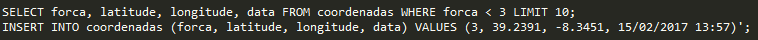
\includegraphics[width=14.4cm]{sql}
	\caption{Exemplo de código SQL}
	\label{fig:sql}
\end{figure}

\section{Linguagem de marcação - HTML}
\label{sec:html}

HTML é uma linguagem de marcação utilizada para a construção de páginas \emph{web}, que são interpretadas pelo navegador.
O navegador pode ter acesso ao ficheiro se ele estiver alocado num servidor ou num ficheiro local, transformando-o numa página \emph{web} totalmente navegável.
Esta linguagem torna possível a utilização de imagens, texto e vídeos numa página \emph{web}, bem como formulários interativos.
As marcações de HTML são maioritariamente denominadas \emph{tags}, um tipo de dados que recebe parâmetros de entrada e os molda, consoante a sua função.
Estas \emph{tags} costumam ser apresentadas em pares, como ``<h1>'' e ``</h1>'' que afetam todo o código que se encontre entre elas, neste caso, tornando o texto normal em cabeçalho de nível 1, mas também podem ser individuais, como ``<img>'', que determina uma imagem e todos os seus atributos.
Outro aspeto importante em HTML é a declaração da linguagem a utilizar.
Apesar da página ter a extensão HTML, ela suporta outras linguagens como PHP, JavaScript e também SQL, tornando esta linguagem muito mais completa e diversificada, sendo assim possível utilizar determinadas linguagens nos pontos fortes de cada uma.

\begin{figure}[hbtp]
	\centering
	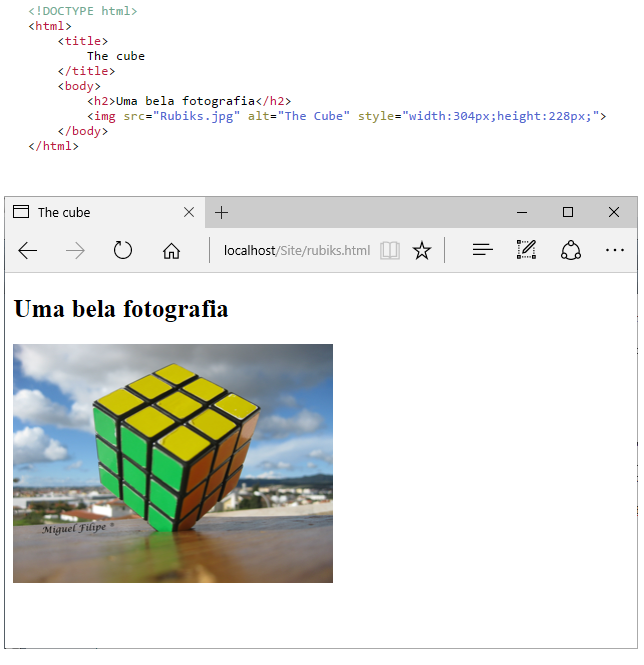
\includegraphics[width=14.4cm]{hello}
	\caption{Exemplo de código HTML e o resultado num browser}
	\label{fig:hello}
\end{figure}

Na figura \ref{fig:hello} é possível distinguir várias secções do código:
O texto entre ``<html>'' e ``</html>'' descreve a página e a linguagem em que deve ser interpretado.
Entre ``<title>'' e ``</title>'' vem o título da página que apenas aparece como título do navegador.
Já em ``<body>'' e ``</body>'' está o texto visível, que aparece na execução da página.
``< h2>'' e ``</h2>'' representam um cabeçalho de nível 2 e <img ... > é uma imagem, com os seus atributos declarados.